\documentclass[12pt]{article}

\usepackage{sbc-template}
\usepackage{graphicx}
\usepackage[hyphens]{url}
\makeatletter\g@addto@macro{\UrlBreaks}{\do\_}\makeatother
\usepackage[utf8]{inputenc}
\usepackage[T1]{fontenc}
\usepackage[english]{babel}
\usepackage{amsmath}
\usepackage{booktabs}
\usepackage{array}
\usepackage{enumitem}
\usepackage{xcolor}
\usepackage{tikz}
\usetikzlibrary{positioning,arrows.meta,fit}
\usepackage{pgfplots}
\pgfplotsset{compat=1.18}
\usepgfplotslibrary{groupplots}

% Colors of the IAês site.
\definecolor{excess}{HTML}{D84925}
\definecolor{ptcol}{HTML}{0A96AF}
\definecolor{encol}{HTML}{3853B6}
\definecolor{ink}{HTML}{1C1A17}
\definecolor{ink2}{HTML}{4F4D48}
\definecolor{gridline}{HTML}{E1DFDB}
\definecolor{content}{HTML}{8C8A85}
\definecolor{ambiguous}{HTML}{D3D0CB}

% A word mentioned as a word.
\newcommand{\w}[1]{\textit{#1}}
\newcommand{\repo}{\url{https://github.com/ArthurSudbrackIbarra/Trab-BIIAP}}
\newcommand{\site}{\url{https://arthursudbrackibarra.github.io/Trab-BIIAP/}}

\sloppy

\title{Is AI \textit{delving} into Brazilian science? The lexical footprint\\
  of LLM chatbots in Portuguese and English abstracts}

\author{Arthur Sudbrack Ibarra\inst{1},\\
  Rodrigo Coelho Barros\inst{1} (advisor),
  Lucas Silveira Kupssinskü\inst{1} (co-advisor)}

\address{Programa de Pós-Graduação em Ciência da Computação (PPGCC)\\
  Pontifícia Universidade Católica do Rio Grande do Sul (PUCRS)\\
  Porto Alegre, RS, Brazil
  \email{arthur.ibarra@edu.pucrs.br}
}

\begin{document}

\maketitle

\begin{abstract}
  Chatbots built on large language models (LLMs) have favorite words, and since ChatGPT appeared,
  words such as \emph{delves} have become far more common in scientific abstracts. We looked for
  this footprint in 195,600 Portuguese and English abstracts published by SciELO Brazil journals
  from 2015 to 2026, adapting the excess-vocabulary method of Kobak et al.\ to a smaller, bilingual
  corpus. From 2018 to 2022, no more than six style words a year rose above their trend in either
  language. In 2025, 108 did in
  English and 69 in Portuguese, and from them we estimate that at least 17\% of the English and 13\%
  of the Portuguese abstracts of that year went through an LLM. Within the same papers, the English
  abstract did not gain clearly more of these marker words than the Portuguese one. Most Portuguese
  markers are translations of English ones, a sign that chatbots carry their English word choices
  into Portuguese. In an experiment, ChatGPT and Gemini added about five markers to each English
  abstract they polished. The data can be explored on IAês, an open bilingual website.
\end{abstract}

%%%%%%%%%%%%%%%%%%%%%%%%%%%%%%%%%%%%%%%%%%%%%%%%%%%%%%%%%%%%%%%%%%%%%%%%%%%%%%%%%%%%%%%%%%%%%%%%%%
\section{Introduction}
\label{sec:intro}

Since OpenAI released ChatGPT on 30 November 2022 \cite{openai2022chatgpt}, chatbots based on large
language models (LLMs) have become everyday writing tools in research. In a 2025 survey of more
than 5,000 researchers, about 28\% had used AI to edit a paper, and most of those who had used AI
had not disclosed it \cite{kwon2025ok}. Journals and publishers reacted early. They ruled that an
LLM cannot be listed as an author and that its use must be disclosed \cite{nature2023tools}, but
disclosure has lagged behind use: in 2023, at least 60,000 papers, slightly over 1\% of all
articles, already showed signs of LLM use, while explicit disclosures were very rare
\cite{gray2024contamination}.

When authors do not report that a chatbot helped them, the text itself can give it away. Chatbots
favor certain words, and as more people use them, those words become more common across the
literature. In PubMed abstracts, \w{delves} and \w{underscores} rose far above their trend after
2022, much as \w{covid} had in 2020. From this \emph{excess vocabulary}, Kobak et al.\ estimated that
at least 13.5\% of the abstracts of 2024 had been processed with an LLM \cite{kobak2025delving}.
Later studies found similar traces in computer science and in full texts
(Section~\ref{sec:related}), but almost all of this evidence comes from texts written in English.

Brazil is a good place to ask whether the trail looks the same in another language. In SciELO, the
open-access library that publishes the country's journals online, the share of documents available
in English rose from 37\% in 2003 to 76\% in 2022 \cite{packer2024multilingualism}. Many articles
therefore carry two abstracts, one in Portuguese and one in English, and the English one is usually
the harder of the two to write. Researchers who learned
English as a second language work under steady pressure to publish in it \cite{meneghini2007there}.
They can spend up to 51\% more time writing a paper, and journals reject their papers because of
the language about 2.5 times as often \cite{amano2023manifold}. Chatbots promise to lower that cost
\cite{berdejoespinola2023ai}, and their use for writing has indeed grown fastest in countries with
lower English proficiency \cite{liu2025aiassisted}.

Brazilian institutions have started to set rules for this use. SciELO asks authors to report any
use of AI tools \cite{scielo2023guia}, and CNPq lists the declaration of any use of generative AI
among the integrity guidelines for the research it funds \cite{cnpq2026portaria}. Yet, to our
knowledge, no study has looked for excess vocabulary in Portuguese or in SciELO. This study
therefore asks:
\emph{have LLM chatbots left a measurable lexical footprint in the abstracts of Brazilian journals
indexed in SciELO, is that footprint larger in the English abstract than in the Portuguese abstract
of the same paper, and is it made of the same words in both languages?}

Each part of the question has an expected answer, which we state as a hypothesis.
\begin{itemize}[nosep, leftmargin=1.1cm, labelsep=0.3cm, itemsep=1pt, topsep=2pt]
  \item[\textbf{H1}] Since 2023, some \emph{style words}, words that reflect how authors write and
    not what they study, appear above their pre-2023 trend in both languages, as they did in PubMed.
  \item[\textbf{H2}] The footprint is larger in the English abstract than in the Portuguese abstract
    of the same paper. We expected this for three reasons: authors are more likely to seek help in
    the language they master less, chatbots learn mostly from English text, and in Korean journals
    the English abstracts changed earlier and more than the Korean ones
    \cite{koo2026lexical,lee2026korean}.
  \item[\textbf{H3}] The Portuguese words that rose above their trend are mostly style words, and
    they differ from the English ones, as would happen if chatbots had a separate style in each
    language.
\end{itemize}
The second half of H3 was open to doubt from the start: in a study of news in 34 languages, GPT-4.1
overused verbs meaning \w{emphasize} in 24 of them \cite{juzek2026crosslingual}. If chatbots behave
the same way in scientific abstracts, most of the Portuguese words should be translations of the
English ones.

Our objective is to measure this footprint year by year in both languages, in abstracts published
from 2015 to 2026, and to compare the two abstracts of the same papers, as \cite{lee2026korean} did
for Korean. We also test whether the Portuguese words are translations of English ones, ask three
current chatbots to rewrite abstracts written before ChatGPT, and present IAês, an open bilingual
website for exploring the data. The code and the data are open as well.
Section~\ref{sec:foundations} introduces the concepts the study relies on,
Section~\ref{sec:related} reviews related work, Section~\ref{sec:method} describes the data and
methods, Section~\ref{sec:results} presents and discusses the results, and
Section~\ref{sec:conclusion} concludes with the benefits and impacts of AI in this context.

%%%%%%%%%%%%%%%%%%%%%%%%%%%%%%%%%%%%%%%%%%%%%%%%%%%%%%%%%%%%%%%%%%%%%%%%%%%%%%%%%%%%%%%%%%%%%%%%%%
\section{Theoretical foundations}
\label{sec:foundations}

\subsection{Language models and chatbots}

A language model writes one token at a time, a token being a word or a piece of a word. At each
step it assigns a probability to every possible next token, given the text so far, and picks one.
After ``This study aims to'', for example, \w{investigate} gets a high probability and \w{banana}
almost none. Current models are built on the transformer architecture \cite{vaswani2017attention}
and learn these probabilities from huge amounts of text. A chatbot such as ChatGPT is a model of
this kind that received extra training to follow instructions. It is first shown examples of
requests with good answers (instruction tuning) and then adjusted toward the answers that human
raters prefer (reinforcement learning from human feedback, or RLHF) \cite{ouyang2022training}. This
extra training makes a chatbot useful for editing and translating on request, and it may also shape
the way the chatbot writes, as discussed next.

\subsection{Why chatbots favor certain words}
\label{sec:vocab}

Training on human preferences narrows what a model writes: tuned models produce less varied outputs
than the models they started from \cite{kirk2024understanding}. Some words stand out. \w{Delve},
\w{intricate} and \w{underscore} appear far more often in LLM output than in human text, and the
cause is still unclear. One study of this overuse found no evidence that the training data or the
model architecture explain it, and mixed evidence that learning from human feedback does
\cite{juzek2025delve}.

These habits are not fixed. Each model has its own, distinct enough for a classifier to tell which
of five chatbots wrote a text 97\% of the time \cite{sun2025idiosyncrasies}, and the favored words
change from one model generation to the next, which makes detection tools fail after a change of
model \cite{nakajima2026turnover}. People react as well: they pick the words up in their own speech
\cite{yakura2024empirical}, or avoid them once they become known as signs of AI, as happened to
\w{delve} in early 2024 \cite{geng2025coevolution}. Any list of words that mark chatbot text
therefore has to be renewed from time to time.

\subsection{Excess vocabulary}
\label{sec:excess-theory}

To say that a word is used more than it should be, we need an idea of how often it would have been
used otherwise. Corpus linguistics has long compared word frequencies across corpora, that is,
large collections of texts, to find what sets one of them apart \cite{rayson2000comparing}. Kobak et
al.\ combined this idea with the logic of excess mortality \cite{kobak2025delving}. In epidemiology,
the deaths above the number expected from earlier years measure the toll of an event such as a
pandemic \cite{karlinsky2021tracking}. In the same way, the uses of a word above the number expected
from earlier years measure how much an event, here the arrival of chatbots, changed the way people
write.

For a word and a year $Y$, let $p_Y$ be the share of that year's abstracts that contain the word.
The expected share $q_Y$ extends the trend of two earlier years:
\begin{equation}
  q_Y = p_{Y-2} + 2\,\max\left(p_{Y-2} - p_{Y-3},\; 0\right).
  \label{eq:expected}
\end{equation}
Suppose a word appeared in 1.0\% of the abstracts of 2021 and in 1.2\% of those of 2022. It was
gaining 0.2 points a year, so for 2024, two years later, we expect $1.2 + 2 \times 0.2 = 1.6\%$.
Two details of the formula matter. It skips the year right before $Y$, so that the trend for 2024
comes from 2021 and 2022, before chatbots were in wide use. And it never assumes a decline: if the
word was losing ground, the formula expects it to stay where it was, which makes an excess harder
to find, not easier.

A word is in excess when $p$ clearly exceeds $q$. The distance can be measured as a gap,
$\delta = p - q$, or as a ratio, $r = p/q$. If the word of the example reached 4\% in 2024, its gap
would be 2.4 points and its ratio 2.5. The gap suits common words. The ratio suits rare ones, whose
share can multiply several times and still move by only a fraction of a point.

Not every excess word points to a chatbot. In 2020, \w{covid} and \w{pandemic} rose far above any
trend because the subject of research had changed. The method therefore separates \emph{content
words}, which follow what researchers study, from style words, which follow how they write, and
attributes to LLMs only the style words that rose after 2022. We call these words \emph{markers}.

\subsection{From excess words to a share of abstracts}
\label{sec:bound-theory}

Excess words show that something changed, but not how many abstracts the change reached. A simple
argument gives at least a minimum. Take a set of markers, and let $p$ be the share of a year's
abstracts that contain at least one of them and $q$ the share expected without LLMs. If a share $f$
of the abstracts went through an LLM, and a share $s$ of those contain a marker, then
\begin{equation}
  p = (1-f)\,q + f\,s
  \quad\Longrightarrow\quad
  \Delta = p - q = f\,(s - q) \le f,
  \label{eq:bound}
\end{equation}
so the gap $\Delta$ can never exceed $f$. If 50\% of the abstracts of a year contain a marker where
35\% were expected, at least 15\% of them went through an LLM. The true share is usually well above
the gap, because many processed texts contain no marker ($s < 1$) and some unprocessed texts contain
one anyway ($q > 0$). Since $s$ cannot exceed 1, the same equation also gives a tighter bound,
$f \ge \Delta/(1-q)$ \cite{holzwarth2026most}, which in the example is $15/65$, or 23\%. Both bounds
rest on one assumption, that the texts no LLM touched keep following the trend. They would overstate
$f$ if authors picked up the marker words on their own (Section~\ref{sec:alternatives}).

Estimating $\Delta$ has one trap. Markers are picked because they rose, and some of them rose partly
by chance. If the same abstracts serve both to pick the markers and to measure the gap, that luck is
counted as signal and the gap comes out too large, a form of circular analysis
\cite{kriegeskorte2009circular}. The remedy is to pick the markers on one half of the data, measure
the gap on the other half, and then swap the halves, a procedure known as cross-fitting
\cite{chernozhukov2018double}.

The bound describes a population of texts and says nothing about any single one. We see this as an
advantage. Tools that try to judge single texts are unreliable \cite{weberwulff2023testing}, and
they flag, on average, 61\% of essays by non-native English speakers as written by AI
\cite{liang2023gpt}.

\subsection{Two abstracts of the same paper}
\label{sec:paired-theory}

The bilingual abstracts of SciELO allow a sharper comparison between languages. The Portuguese and
English abstracts of a paper describe the same work and share authors, journal, field and year, so
comparing them holds all of these fixed and leaves language as the main difference. If authors used
chatbots mostly for the English version, the share of English abstracts with a marker would rise
more than the share of Portuguese abstracts with one in the same papers. Subtracting one rise from
the other gives a difference in differences \cite{angrist2009mostly}: if the English share rose 15
points and the Portuguese share 10, the estimate is 5 points, and whatever affected both versions
alike cancels out. The comparison is fair only if the markers of the two languages are equally
likely to catch an edit, a condition that the experiment of Section~\ref{sec:experiment} lets us
examine. The design also cannot show who produced each version, whether the authors, a translator
or a tool.

%%%%%%%%%%%%%%%%%%%%%%%%%%%%%%%%%%%%%%%%%%%%%%%%%%%%%%%%%%%%%%%%%%%%%%%%%%%%%%%%%%%%%%%%%%%%%%%%%%
\section{Related work}
\label{sec:related}

Most estimates of LLM use in science come from English texts and follow one of three approaches.
The first counts the words that rose above their trend, as Kobak et al.\ did for PubMed
\cite{kobak2025delving} and a later study did for linguistics \cite{botes2026initial}. The second
tracks a fixed list of words known to be favored by LLMs, such as twelve terms followed across six
databases \cite{kousha2026much}. The third compares the distribution of words in a corpus with that
of known human and LLM texts to estimate how much text was modified
\cite{liang2025quantifying,geng2024transforming}. Recent studies take these ideas to full texts
\cite{siler2026diffusion,holzwarth2026most}. Table~\ref{tab:related} compares what the main studies
do and what they estimate. Some of them also compare countries. In PubMed, for instance, the excess
was about four times larger for papers from China, South Korea and Taiwan than for papers from the
United Kingdom and Australia \cite{kobak2025delving}. But all these authors write in English, so
such comparisons cannot show how the footprint differs between two languages.

Outside English, the evidence is thin. In about 880,000 abstracts of Korean humanities and social
science journals, English style words such as \w{additionally} rose sharply from 2023 on, and
Korean expressions less so \cite{koo2026lexical}. A preprint adapted the excess-vocabulary method to
Korean, a language in which words take many forms, and found the excess in the English abstracts a
year before it reached the Korean abstracts of the same papers \cite{lee2026korean}. In news,
AI-associated words rose in 26 of 34 languages \cite{juzek2026crosslingual}. For Portuguese, we
found two studies. One measured shorter abstracts with simpler syntax and more varied vocabulary in
Brazilian computing venues in 2024 and 2025, using text metrics instead of marker words
\cite{lobo2026evolucao}. The other tested AI detectors on scientific texts
\cite{candido2025analise}. We found no excess-vocabulary study of Portuguese or of SciELO.

Our design is closest to that of the Korean preprint. Like it, we compare the two abstracts of the
same papers, choose the markers apart from the texts we measure, and have chatbots rewrite
abstracts. We add a Portuguese corpus, confidence intervals for the difference between the two
languages, and a test of whether the markers of one language translate those of the other.

\begin{table}[t]
  \centering
  \caption{The main studies of LLM use in scientific texts, and this study. Pairs: compares the two
    abstracts of the same papers. Held out: picks the markers apart from the texts it measures. LLM
    texts: has LLMs write or rewrite texts to test the measure. Placebo: tests the estimate on years
    before ChatGPT. Transl.: tests whether markers translate across languages. Main estimate: share
    of abstracts with LLM use, unless stated. CS: computer science; PMC: PubMed Central.}
  \label{tab:related}
  \footnotesize
  \setlength{\tabcolsep}{1.9pt}
  \begin{tabular}{>{\raggedright\arraybackslash}p{3.55cm}>{\raggedright\arraybackslash}p{1.6cm}ccccc>{\raggedright\arraybackslash}p{4.4cm}}
    \toprule
    Study & Languages & Pairs & \shortstack{Held\\out} & \shortstack{LLM\\texts} & Placebo
      & Transl. & Main estimate \\
    \midrule
    \cite{kobak2025delving} & EN & -- & no & no & no & -- & $\ge$13.5\% (PubMed, 2024) \\
    \cite{liang2025quantifying} & EN & -- & -- & yes & no & -- & Up to 22\% of CS sentences \\
    \cite{gray2024contamination} & EN & -- & partly & no & no & -- & Over 1\% of articles (2023) \\
    \cite{geng2024transforming} & EN & -- & yes & yes & no & -- & LLM impact near 35\% (CS) \\
    \cite{holzwarth2026most} & EN & -- & partly & no & no & -- & 77\% of full texts (PMC, 2025) \\
    \cite{koo2026lexical} & KO, EN & no & no & no & no & no & No share \\
    \cite{lee2026korean} & KO, EN, VI & yes & yes & yes & yes & no & $\ge$20.6\% (Korean, 2025) \\
    \cite{lobo2026evolucao} & PT & -- & -- & no & no & -- & No share \\
    This study & PT, EN & yes & yes & yes & yes & yes & $\ge$17.3\% EN, $\ge$12.7\% PT (2025) \\
    \bottomrule
  \end{tabular}
\end{table}

%%%%%%%%%%%%%%%%%%%%%%%%%%%%%%%%%%%%%%%%%%%%%%%%%%%%%%%%%%%%%%%%%%%%%%%%%%%%%%%%%%%%%%%%%%%%%%%%%%
\section{Methodology}
\label{sec:method}

The study combines three sources of evidence, shown in Figure~\ref{fig:pipeline}: the full Crossref
corpus, a sample of papers with abstracts in both languages, and a rewriting experiment. The code,
the tables it produces, the prompts, the word labels and the chatbots' replies are in the project's
repository\footnote{\repo}, so every number in this paper can be traced and recomputed. Each
analysis step runs in minutes on a desktop computer, and the data collection can be repeated from
the public SciELO and Crossref APIs. The same data are presented on IAês\footnote{\site. The name
joins \emph{IA}, Portuguese for AI, and \emph{-ês}, the ending of language names such as
\emph{português} and of words such as \emph{juridiquês} (legalese).}, a website in English and Portuguese where readers can follow any word over
time, compare fields, read the sampled papers and the experiment's texts side by side, and see
which marker words a text of their own contains (Figure~\ref{fig:site-time-machine}).

\begin{figure}[t]
  \centering
  % Figure 1: data, measurement and analyses.
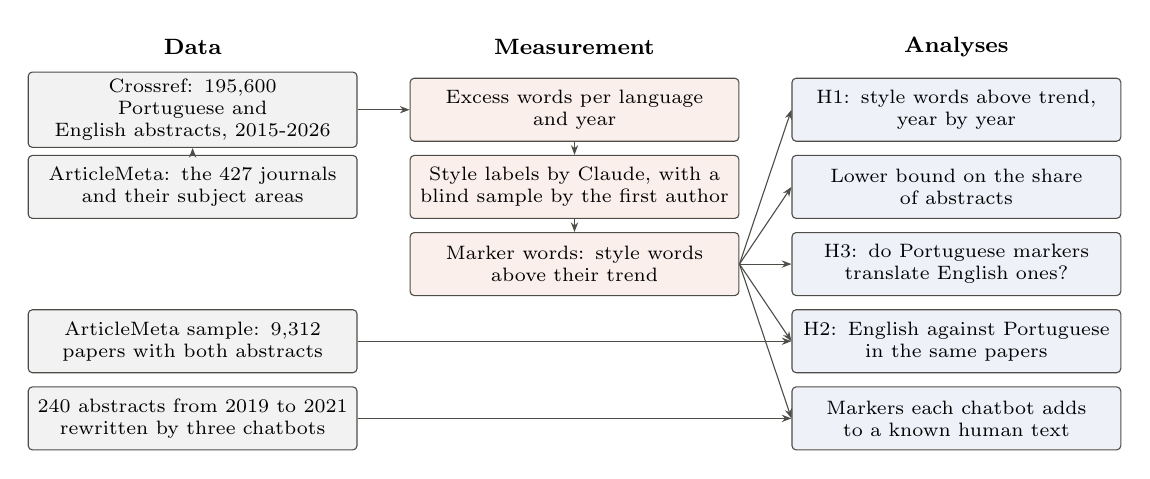
\begin{tikzpicture}[
    font=\scriptsize,
    box/.style={draw=ink2, rounded corners=1.5pt, align=center, text width=4.0cm,
      inner sep=2.5pt, minimum height=8mm},
    data/.style={box, fill=black!5},
    proc/.style={box, fill=excess!9},
    result/.style={box, fill=encol!8},
    arr/.style={-{Stealth[length=3.5pt]}, ink2, thin},
  ]
  \node[font=\footnotesize\bfseries] at (0, 0.8) {Data};
  \node[font=\footnotesize\bfseries] at (4.85, 0.8) {Measurement};
  \node[font=\footnotesize\bfseries] at (9.7, 0.8) {Analyses};

  \node[data] (crossref) at (0, 0) {Crossref: 195,600 Portuguese and\\English abstracts, 2015-2026};
  \node[data] (journals) at (0, -0.98) {ArticleMeta: the 427 journals\\and their subject areas};
  \node[data] (pairs) at (0, -2.94) {ArticleMeta sample: 9,312\\papers with both abstracts};
  \node[data] (experiment) at (0, -3.92) {240 abstracts from 2019 to 2021\\rewritten by three chatbots};

  \node[proc] (excess) at (4.85, 0) {Excess words per language\\and year};
  \node[proc] (labels) at (4.85, -0.98) {Style labels by Claude, with a\\blind sample by the first author};
  \node[proc] (markers) at (4.85, -1.96) {Marker words: style words\\above their trend};

  \node[result] (h1) at (9.7, 0) {H1: style words above trend,\\year by year};
  \node[result] (bound) at (9.7, -0.98) {Lower bound on the share\\of abstracts};
  \node[result] (h3) at (9.7, -1.96) {H3: do Portuguese markers\\translate English ones?};
  \node[result] (h2) at (9.7, -2.94) {H2: English against Portuguese\\in the same papers};
  \node[result] (exp) at (9.7, -3.92) {Markers each chatbot adds\\to a known human text};

  \draw[arr] (crossref) -- (excess);
  \draw[arr] (journals.north) -- (crossref.south);
  \draw[arr] (excess) -- (labels);
  \draw[arr] (labels) -- (markers);
  \draw[arr] (markers.east) -- (h1.west);
  \draw[arr] (markers.east) -- (bound.west);
  \draw[arr] (markers.east) -- (h3.west);
  \draw[arr] (markers.east) -- (h2.west);
  \draw[arr] (markers.east) -- (exp.west);
  \draw[arr] (pairs) -- (h2);
  \draw[arr] (experiment) -- (exp);
\end{tikzpicture}

  \caption{Overview of the study. The Crossref corpus gives the measures by language (H1, the lower
    bound and H3), a sample of papers with both abstracts gives the same-paper test (H2), and a
    rewriting experiment shows what chatbots add to texts written before ChatGPT.}
  \label{fig:pipeline}
\end{figure}

\subsection{Data}
\label{sec:data}

SciELO Brazil had 427 journals when we collected the data. SciELO assigns each journal to one or
more of eight subject areas, and we took both the list of journals and their areas from SciELO's
ArticleMeta API. The abstracts themselves come from Crossref, the registry where journals deposit
the metadata of their articles. On 30 October 2026 we downloaded every article of these journals
published from 2015 to 2026 that had an abstract, 214,252 records in all. We date each article by
the earliest publication date that Crossref records, so 2026 is a partial year throughout this
paper. Crossref has two drawbacks for our purposes. It usually keeps a single abstract per article,
in the language of the article, which suits an analysis by language but cannot pair the two
abstracts of one paper. And its coverage is uneven: some journals deposit no abstracts, and others
deposited them for a few years, stopped and started again, a problem we return to in
Section~\ref{sec:excess-method}.

Before counting words, we cleaned the corpus with filters close to those of Kobak et al. We removed
duplicate records, errata and retraction notices, abstracts shorter than 250 or longer than 4,000
characters, abstracts whose function words (articles, prepositions and the like) did not clearly
point to one language, and abstracts with a second abstract or the keywords attached. This left
204,937 usable abstracts from 357 journals: 94,882 in Portuguese, 100,718 in English and 9,337 in
Spanish. We set the Spanish ones aside, so the analyses use 195,600 abstracts. As in Kobak et al.,
a word is any sequence of four or more letters, which leaves out most function words. We lowercase
the text, keep accented letters, split words at hyphens and digits, and count each word at most
once per abstract. Words are counted in the form in which they appear, so \w{delve}, \w{delves} and
\w{delving} are three different words.

To pair the two languages, we turned to ArticleMeta, which keeps every abstract of an article. It
is slow, taking one to three seconds per article, so we drew a random sample of 1,300 articles per
year from all the journals. After the same cleaning,
9,312 papers from 315 journals had a usable abstract in both Portuguese and English, between 695
and 865 per year.

\subsection{Excess words}
\label{sec:excess-method}

For each language, year and word, we computed the observed share $p$ and the expected share $q$ of
Section~\ref{sec:excess-theory}. The expected share depends on which earlier years define the trend,
and we used two baselines for two purposes. The \emph{rolling baseline} applies
Equation~\ref{eq:expected} to every year, so each year, before or after ChatGPT, is compared with a
trend over the same span. This makes the years before 2023 a fair reference for how many excess
words appear when there are no chatbots, and we used it to count excess words year by year (H1).
Its weakness is that, for 2025 and 2026, the trend already includes years with ChatGPT, which makes
their counts conservative. The \emph{fixed baseline} avoids this by predicting every year after
2022 from 2021 and 2022 alone, as $q_Y = p_{2022} + (Y - 2022)\max(p_{2022} - p_{2021}, 0)$. We used
it for the lower bound, for the marker sets of the same-paper test and for the site.

Our corpus has between 5,000 and 14,000 usable abstracts per language and year, about a hundred
times fewer than PubMed. In a corpus this small, chance and changes in the corpus itself can easily
pass for excess, so we made three changes to the method.

The first concerns which journals are compared. Journals enter and leave Crossref, and a word can
seem to rise only because a journal that uses it started to deposit abstracts. Without a
correction, dozens of such words appear in years before ChatGPT. Each comparison therefore uses a
balanced panel, made of the journals with at least five usable abstracts in the language in every
year involved.

The second concerns length. Abstracts got longer over the period (English abstracts had 85 distinct
words on average in 2022 and 99 in 2026), and a longer abstract is more likely to contain any given
word. We sorted the abstracts of the baseline years into ten length bands (deciles) and reweighted
each later year so that every band counts as much as it did in the baseline. A word cannot rise
just because the texts grew.

The third makes the selection stricter. An excess word had to appear in at least ten abstracts of
the year and pass three tests. It had to meet the thresholds of Kobak et al., a gap $\delta > 0.01$
or a ratio $r > 2^{-\log_{10}(p)/4}$, a bar that falls as the word gets more common, from 2 for
$p = 10^{-4}$ to 1.41 for $p = 10^{-2}$.\footnote{Kobak et al.\ print this threshold without the
minus sign, and we follow their code.} Its gap had to pass a $z$ test that accounts for the noise of
both the year and the baseline years. Thousands of words are tested in each language and year, and
some would pass by chance alone, so we applied the Benjamini-Hochberg correction, which keeps the
expected share of false alarms among the selected words at 5\% \cite{benjamini1995controlling}. And
the word had to be used by at least five journals, none of them holding more than half of its uses.
This last condition, which we call the spread test, removes words that a single journal brings in,
for instance with a special issue.

\subsection{Style labels}
\label{sec:labels}

To tell style words from content words, we asked Claude Opus 5.5 to label as style, content or
ambiguous each of the 1,682 words that came out as excess in any of our runs (any year, language,
baseline or half of the corpus). The words came in alphabetical order and without their year, so
the model could not tell which period a word belonged to. To check the labels, the first author
labeled a random sample of 100 words per language without seeing Claude's, using only style and
content. The two agreed on 72\% of the Portuguese words and 67\% of the English ones, with a Cohen's
$\kappa$, a measure of agreement that discounts chance, of 0.50 and 0.36
\cite{cohen1960coefficient}. More than half of the disagreements (36 of 61) were words that Claude
had called ambiguous and the first author called style. Where Claude did choose style or content,
the two agreed on 92\% and 91\% of the words. Claude's labels, and the marker sets built from them,
therefore lean conservative. For the 200 sampled words, the first author's label replaced Claude's.

\subsection{Lower bound}
\label{sec:bound-method}

The lower bound of Section~\ref{sec:bound-theory} needs a set of marker words for each language and
year. For each year from 2023 on, the candidates are that year's excess style words under the fixed
baseline. Following Kobak et al., we kept only the candidates rarer than a threshold $T$, since rare
words are more specific to LLM text. We tried thresholds from 0.2\% to 10\% of the abstracts, and no
threshold at all, and kept the one that made the gap $\Delta$ largest. This choice looks at the
data, which is the trap described in Section~\ref{sec:bound-theory}, so we cross-fitted the
estimate. We split the abstracts at random into two halves by DOI, chose the markers and the
threshold on one half and measured $\Delta$ on the other, then swapped the halves and averaged the
two results, much as \cite{lee2026korean} did with a split by journal. The standard errors come
from a bootstrap \cite{efron1979bootstrap}: we recomputed the gap on 1,000 random resamples of the
journals of the panel, with the marker sets held fixed. We resampled journals, not abstracts,
because the abstracts of one journal share editors, rules and topics.

Besides the cross-fitted gap, we report the tighter bound $\Delta/(1-q)$ and the same-data estimate,
in which the markers are chosen and measured on all abstracts, as Kobak et al. did. A placebo checks
that the procedure stays quiet when it should. We took the same-data markers of each year and
measured their gap six years earlier, in 2017 to 2020, with 2015 and 2016 as the baseline. With no
chatbots in those years, the gap should be near zero. Three
further checks counted ambiguous words as style, required 20 abstracts and 10 journals per excess
word, and replaced the two-year trend with a linear trend fitted to 2017-2022, since a trend
extended from two years is noisy in a corpus of this size.

\subsection{Same papers (H2)}
\label{sec:h2-method}

For the same-paper test, we checked, for each paper of the ArticleMeta sample, whether its English
abstract contains an English marker and whether its Portuguese abstract contains a Portuguese one.
The markers are the cross-fitted sets of the lower bound, taken from the Crossref half that the
paper's DOI does not belong to, so a paper never helped choose the markers that judge it. The test
covers 2025 and 2026 only. These are the years with at least ten markers per half in both
languages, since the Portuguese sets of 2023 and 2024 have one word or none.

With fewer than 900 papers a year, a trend fitted on two years would be too noisy, so the expected
share is simply that of 2021 and 2022, standardized to the length quintiles (five length bands) of
those years. The estimate is the difference in differences of Section~\ref{sec:paired-theory}, that
is, how much more the English share rose than the Portuguese share in the same papers. Its 95\%
intervals and one-sided $p$-values come from 2,000 bootstrap resamples of the journals, each with
all its papers of every year. As a placebo, we applied the same sets and span to 2015-2016 and
2019-2020.

Three further analyses help to read the result. For the timing, we applied the 2025 sets to every
year from 2015 to 2026. For robustness, we dropped the length standardization, used 2019 to 2022 as
the baseline and used the same-data marker sets. And to see whether the Portuguese markers could
simply come from translating an edited English abstract, we measured their rise in the papers whose
English abstract has no marker and recomputed the lower bound with only the Portuguese markers that
have no English counterpart in the H3 test, described next.

\subsection{Cross-language test (H3)}
\label{sec:h3-method}

If the Portuguese markers were mostly translations of English ones, a Portuguese marker should
translate into an English marker more often than a comparable Portuguese word that never rose. The
markers of this test are the excess style words of 2024 to 2026 under either baseline, 349 in
Portuguese and 437 in English. Each marker gets a control: the word of the same
language with the closest frequency in 2021-2022 that was never in excess and that Claude, given
the same instructions, labels as style. Claude gave the dictionary form of every marker (\w{delve}
for \w{delves}) and translated markers and controls, shuffled together, into the other language,
listing the usual translations of each word. We say that a word \emph{hits} when one of its
translations, in dictionary form, is the dictionary form of a marker of the other language.

Markers and controls come in pairs, so we compared them with an exact one-sided McNemar test
\cite{mcnemar1947note}, which looks only at the pairs in which one of the two words hits and the
other does not. If markers hit significantly more often than their controls, the claim of H3 that
the two sets differ fails. Because the inflected forms of one word count as separate markers, we
repeated the test with one pair per dictionary form, keeping the most frequent marker of each.
Claude translated each word without context, so the first author checked a random sample of 50
translated words, markers and controls together, without knowing which was which.

\subsection{Rewriting experiment}
\label{sec:experiment-method}

The analyses above show that the vocabulary changed, but not how much a single use of a chatbot
changes a text. To see this, we gave chatbots texts whose history we know and counted the markers
they added. We sampled abstracts published from 2019 to 2021, before ChatGPT, for three tasks. Two
asked a chatbot to improve the writing of an abstract, one in Portuguese and one in English. The
third asked it to translate a Portuguese abstract into English, with the authors' own English
abstract as the human reference. Each task has 80 abstracts, ten per subject area, and no paper
appears in two tasks. Each prompt was written in the language of the source abstract and asked for
an abstract ready to submit to a journal, with the meaning, data and numbers of the original. Three
chatbots did every task with the same prompts, in batches of ten abstracts per new conversation, on
30 and 31 October 2026: ChatGPT (GPT-6 Luna, the model of the free plan, in temporary chats),
Gemini 3.6 Flash (Google AI Pro plan) and Claude Sonnet 5.5 (through the command-line mode of
Claude Code, without tools).

For each text, we counted the H3 markers before and after the chatbot's pass, with intervals from
resampling the texts. We also listed the words each model adds or drops, counting a word when the
number of texts that contain it changes by at least 4 of 80. To connect the experiment with the
same-paper test, we checked whether each text contains a marker of the cross-fitted sets of 2025
and 2026.

%%%%%%%%%%%%%%%%%%%%%%%%%%%%%%%%%%%%%%%%%%%%%%%%%%%%%%%%%%%%%%%%%%%%%%%%%%%%%%%%%%%%%%%%%%%%%%%%%%
\section{Results and discussion}
\label{sec:results}

\subsection{Style words rose above their trend in both languages (H1)}
\label{sec:h1}

Before ChatGPT, few words rose above their trend. From 2018 to 2022, the rolling baseline finds at
most one style word a year in Portuguese and six in English. In 2020 and 2021, content words
outnumber style words among the excess words, and many are about the pandemic, such as \w{covid},
\w{pandemia}, \w{coronavírus} and \w{sars} (Figure~\ref{fig:excess}). From 2023 on, the picture
changes. The number of excess style words grows every year, from 14 in 2023 to 50, 108 and 150 in
English and from 2 to 10, 69 and 126 in Portuguese, and since 2024 style words have outnumbered
content words every year. Against the fixed 2021-2022 baseline, which keeps the years with ChatGPT
out of the trend, the counts of 2025 are larger still: 201 in English and 99 in Portuguese.

\begin{figure}[!htb]
  \centering
  % Figure 2: excess words per year by label, rolling baseline (analysis/report.md).
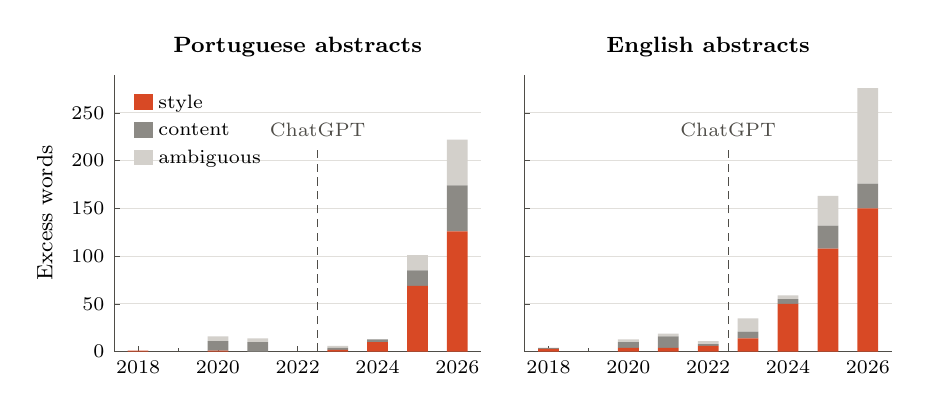
\begin{tikzpicture}
  \begin{groupplot}[
      group style={group size=2 by 1, horizontal sep=0.55cm, y descriptions at=edge left},
      width=0.515\textwidth, height=5.1cm,
      ybar stacked, /pgf/bar width=7.5pt,
      ymin=0, ymax=290, xmin=2017.4, xmax=2026.6,
      xtick={2018,2020,2022,2024,2026}, minor xtick={2019,2021,2023,2025},
      xticklabels={2018,2020,2022,2024,2026},
      ytick={0,50,100,150,200,250},
      tick label style={font=\scriptsize}, label style={font=\footnotesize},
      title style={font=\footnotesize\bfseries, yshift=-3pt},
      axis lines*=left, ymajorgrids, grid style={gridline}, major tick length=2pt,
      minor tick length=1.5pt, axis line style={ink2}, tick style={ink2},
    ]
    \nextgroupplot[title={Portuguese abstracts}, ylabel={Excess words},
      legend style={at={(0.03,0.97)}, anchor=north west, draw=none, fill=none,
        font=\scriptsize, cells={anchor=west}},
      legend image code/.code={\fill[#1] (0cm,-0.08cm) rectangle (0.24cm,0.12cm);}]
    \addplot[fill=excess, draw=none] coordinates
      {(2018,1) (2019,0) (2020,1) (2021,0) (2022,0) (2023,2) (2024,10) (2025,69) (2026,126)};
    \addplot[fill=content, draw=none] coordinates
      {(2018,0) (2019,0) (2020,10) (2021,10) (2022,0) (2023,2) (2024,3) (2025,16) (2026,48)};
    \addplot[fill=ambiguous, draw=none] coordinates
      {(2018,0) (2019,0) (2020,5) (2021,4) (2022,0) (2023,2) (2024,0) (2025,16) (2026,48)};
    \legend{style, content, ambiguous}
    \draw[ink2, densely dashed] (axis cs:2022.5,0) -- (axis cs:2022.5,215)
      node[above, font=\scriptsize, ink2] {ChatGPT};
    \nextgroupplot[title={English abstracts}]
    \addplot[fill=excess, draw=none] coordinates
      {(2018,3) (2019,0) (2020,4) (2021,4) (2022,6) (2023,14) (2024,50) (2025,108) (2026,150)};
    \addplot[fill=content, draw=none] coordinates
      {(2018,1) (2019,0) (2020,6) (2021,12) (2022,2) (2023,7) (2024,5) (2025,24) (2026,26)};
    \addplot[fill=ambiguous, draw=none] coordinates
      {(2018,0) (2019,0) (2020,3) (2021,3) (2022,3) (2023,14) (2024,4) (2025,31) (2026,100)};
    \draw[ink2, densely dashed] (axis cs:2022.5,0) -- (axis cs:2022.5,215)
      node[above, font=\scriptsize, ink2] {ChatGPT};
  \end{groupplot}
\end{tikzpicture}

  \caption{Style words above their trend rose after 2022 in both languages. Excess words per year
    in each language, by label, with the rolling baseline. In 2020 and 2021, content words, many
    about the COVID-19 pandemic, outnumbered style words. 2026 runs through October.}
  \label{fig:excess}
\end{figure}

English moved a year earlier than Portuguese. Part of that lead may come from publication delays,
which differ between journals, since many articles of 2023 were written before ChatGPT. The counts
are also better at comparing years than languages, because the tests depend on how many abstracts a
language has in a year.

The English excess style words of 2024 to 2026 include words known to be overused by chatbots
(Section~\ref{sec:vocab}), such as \w{delves}, \w{underscores} and \w{intricate}, along with others
such as \w{scalable} and \w{outperforming}. Among the Portuguese markers of 2025, the highest ratios
belong to \w{multifacetada} (multifaceted), \w{moldam} (they shape), \w{tensionam} (they strain),
\w{perpetuando} (perpetuating) and \w{exigindo} (demanding). Some of the rises are large. In 2025,
\w{underscore} appeared in 20.7 times as many English abstracts as the 2021-2022 trend predicted,
\w{examines} in 6.4 times as many and the Portuguese \w{crucial} in 5.7 times as many. H1 holds in
both languages.

\subsection{The lower bound reached 13\% to 17\% of the abstracts of 2025}
\label{sec:bound}

How many abstracts do these words represent? Table~\ref{tab:bound} gives the cross-fitted lower
bound. In English, the gap was 0.5 points in 2023, 11.2 in 2024, 17.3 in 2025 and 15.8 in partial
2026. In Portuguese, it stayed near zero until 2024, while the marker sets still had one word or
none, and then reached 12.7 in 2025 and 19.4 in 2026. Put plainly, if the abstracts that no LLM
touched kept to their trend, at least one in six English abstracts and one in eight Portuguese
abstracts of 2025 went through an LLM. The tighter bound $\Delta/(1-q)$ raises these shares to
29.5\% and 22.2\%.

\begin{table}[!htb]
  \centering
  \caption{Lower bound on the share of abstracts processed by an LLM (percent), with the 2021-2022
    baseline. Markers: words chosen on each half of the corpus. Obs. and exp.: observed and expected
    share of abstracts with a marker. Gap and $\Delta/(1-q)$: averages of the two cross-fitted
    halves, $\pm$ standard error from resampling journals. Panel: journals and abstracts of the
    year. Same data: markers chosen and measured on all abstracts. Placebo: the same-data markers
    and span, from 2015-2016.}
  \label{tab:bound}
  \footnotesize
  \setlength{\tabcolsep}{3pt}
  \begin{tabular}{llrrrrrrrr}
    \toprule
    Language & Year & Markers & Obs. & Exp. & Gap & $\Delta/(1-q)$ & Panel & Same data & Placebo \\
    \midrule
    Portuguese & 2023 & 1/0   & 5.5  & 3.8  & $1.8 \pm 0.9$  & 1.8  & 169 / 6,879 & 3.4  & $0.9 \pm 0.6$ \\
               & 2024 & 1/0   & 2.6  & 2.2  & $0.4 \pm 0.7$  & 0.4  & 167 / 6,163 & 6.5  & $-1.4 \pm 1.6$ \\
               & 2025 & 50/34 & 52.5 & 39.8 & $12.7 \pm 1.7$ & 22.2 & 168 / 6,431 & 19.5 & $0.3 \pm 2.6$ \\
               & 2026 & 64/73 & 51.9 & 32.5 & $19.4 \pm 2.9$ & 29.8 & 148 / 5,230 & 26.2 & $0.1 \pm 1.5$ \\
    \midrule
    English    & 2023 & 1/3   & 4.6  & 4.1  & $0.5 \pm 0.9$  & 0.6  & 143 / 7,804 & 5.0  & $0.5 \pm 2.2$ \\
               & 2024 & 23/16 & 46.0 & 34.8 & $11.2 \pm 1.5$ & 17.1 & 142 / 7,418 & 15.2 & $-1.8 \pm 1.7$ \\
               & 2025 & 55/97 & 54.1 & 36.8 & $17.3 \pm 1.6$ & 29.5 & 143 / 8,144 & 22.8 & $0.8 \pm 1.2$ \\
               & 2026 & 99/68 & 55.1 & 39.4 & $15.8 \pm 3.6$ & 27.1 & 131 / 6,606 & 26.9 & $2.1 \pm 1.4$ \\
    \bottomrule
  \end{tabular}
\end{table}

Two results suggest that the bound reflects a real change and not a quirk of the procedure. The
placebo gaps lie between $-1.8$ and 2.1 points, all within two standard errors of zero, so the
procedure finds no jump where none should exist. And the three checks of
Section~\ref{sec:bound-method} keep the bound of 2025 between 12.2\% and 13.9\% in Portuguese and
between 13.5\% and 17.3\% in English.

Cross-fitting matters for the size of the estimate. The same-data estimates run higher, by up to 11
points (English in 2026: 26.9 against 15.8), and this difference is the optimism that cross-fitting
removes. For comparison, the same-data procedure gave at least 13.5\% for PubMed in 2024
\cite{kobak2025delving} and gives 15.2\% for SciELO's English abstracts of 2024, or 11.2\% once
cross-fitted.

\subsection{The English abstracts did not gain clearly more markers (H2)}
\label{sec:h2}

The same papers let us compare the two languages directly, and there the English abstracts did not
gain clearly more markers than the Portuguese ones (Table~\ref{tab:h2}). From 2021-2022 to
2025-2026, the share of English abstracts with an English marker rose 17.5 points, and the share of
Portuguese abstracts with a Portuguese marker rose 14.9 points. The difference, 2.7 points
[$-1.9$, 7.0] ($p = 0.14$), is about the size of the placebo difference, 2.4 [$-1.8$, 6.5], and it
stays between 0.2 and 2.7 points in the three robustness checks. With about 700 papers in each of
these years, the data are compatible both with no difference and with an English lead of up to
about 7 points. We cannot rule out a small lead, but we cannot claim one either.

\begin{table}[!htb]
  \centering
  \caption{Same papers in English and Portuguese: share of abstracts with a marker of their
    language in 2021-2022 and in the year (percent), its rise in points, and how much more the
    English share rose. Brackets: 95\% bootstrap intervals from resampling journals. Placebo: the
    same sets and span applied to 2015-2016 and 2019-2020.}
  \label{tab:h2}
  \footnotesize
  \setlength{\tabcolsep}{3pt}
  \begin{tabular}{lccccrr}
    \toprule
    & \multicolumn{2}{c}{English abstracts} & \multicolumn{2}{c}{Portuguese abstracts} & & \\
    \cmidrule(lr){2-3} \cmidrule(lr){4-5}
    Year & Share & Rise & Share & Rise & Difference & Placebo \\
    \midrule
    2025      & 38.5 $\to$ 53.1 & 14.6 [10.2, 19.0] & 36.8 $\to$ 49.0 & 12.2 [7.8, 16.6]
              & 2.4 [$-3.9$, 8.4] & $-0.6$ [$-6.2$, 5.3] \\
    2026      & 37.7 $\to$ 58.3 & 20.6 [15.6, 25.6] & 30.9 $\to$ 48.5 & 17.6 [12.9, 22.6]
              & 3.0 [$-3.5$, 9.4] & 5.4 [$-0.1$, 10.9] \\
    Both      &                 & 17.5 [13.9, 21.1] &                 & 14.9 [11.8, 17.9]
              & 2.7 [$-1.9$, 7.0] & 2.4 [$-1.8$, 6.5] \\
    \bottomrule
  \end{tabular}
\end{table}

Year by year, the two languages did not always move together (Figure~\ref{fig:same-paper}). With
the 2025 marker sets applied to every year, the yearly differences before 2023 all have intervals
that include zero. In 2024, English abstracts rose 8.6 points and Portuguese ones 1.8, a difference
of 6.8 points [1.1, 12.4]. In 2025 the gap nearly closed, with rises of 14.6 and 12.2 points. In
partial 2026 the 2025 sets put English ahead again, by 9.4 points [2.4, 15.7], while the sets
chosen on 2026 abstracts give a difference of only 3.0 [$-3.5$, 9.4]. We read these yearly leads
with caution, because they come from an exploratory check and have other possible explanations. The
Portuguese vocabulary of chatbots may have changed from year to year, so that the 2025 markers miss
part of the use in 2024 and 2026, and Portuguese words are spread over more inflected forms than
English ones, which may delay their detection.

\begin{figure}[!htb]
  \centering
  % Figure: same papers, 2025 marker sets on every year (analysis/pairs/report.md, every paper).
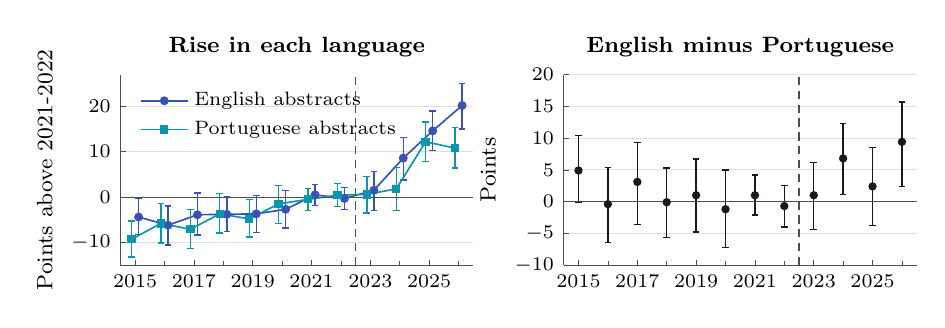
\begin{tikzpicture}
  \begin{groupplot}[
      group style={group size=2 by 1, horizontal sep=1.15cm},
      width=0.5\textwidth, height=4.0cm,
      xmin=2014.5, xmax=2026.5,
      xtick={2015,2017,2019,2021,2023,2025}, minor xtick={2016,2018,2020,2022,2024,2026},
      xticklabels={2015,2017,2019,2021,2023,2025},
      tick label style={font=\scriptsize}, label style={font=\footnotesize},
      title style={font=\footnotesize\bfseries, yshift=-3pt},
      axis lines*=left, ymajorgrids, grid style={gridline}, major tick length=2pt,
      minor tick length=1.5pt, axis line style={ink2}, tick style={ink2},
      error bars/error bar style={line width=0.5pt},
      error bars/error mark options={rotate=90, mark size=1.2pt, line width=0.5pt},
    ]
    \nextgroupplot[title={Rise in each language}, ylabel={Points above 2021-2022},
      ymin=-15, ymax=27, ytick={-10,0,10,20},
      legend style={at={(0.03,0.97)}, anchor=north west, draw=none, fill=none,
        font=\scriptsize, cells={anchor=west}}]
    \addplot[encol, mark=*, mark size=1.3pt, line width=0.6pt,
      error bars/.cd, y dir=both, y explicit] coordinates {
      (2015.12,-4.4) +=(0,4.1) -=(0,3.8) (2016.12,-6.2) +=(0,4.2) -=(0,4.4)
      (2017.12,-3.9) +=(0,4.8) -=(0,4.5) (2018.12,-3.8) +=(0,3.8) -=(0,3.8)
      (2019.12,-3.7) +=(0,4.0) -=(0,4.1) (2020.12,-2.7) +=(0,4.1) -=(0,4.1)
      (2021.12,0.5) +=(0,2.3) -=(0,2.3) (2022.12,-0.3) +=(0,2.4) -=(0,2.4)
      (2023.12,1.5) +=(0,4.2) -=(0,4.5) (2024.12,8.6) +=(0,4.6) -=(0,4.8)
      (2025.12,14.6) +=(0,4.4) -=(0,4.3) (2026.12,20.2) +=(0,4.9) -=(0,5.2)};
    \addplot[ptcol, mark=square*, mark size=1.2pt, line width=0.6pt,
      error bars/.cd, y dir=both, y explicit] coordinates {
      (2014.88,-9.3) +=(0,4.0) -=(0,3.9) (2015.88,-5.8) +=(0,4.4) -=(0,4.3)
      (2016.88,-7.1) +=(0,4.3) -=(0,4.2) (2017.88,-3.7) +=(0,4.5) -=(0,4.2)
      (2018.88,-4.8) +=(0,4.2) -=(0,4.0) (2019.88,-1.5) +=(0,4.1) -=(0,4.3)
      (2020.88,-0.5) +=(0,2.4) -=(0,2.4) (2021.88,0.4) +=(0,2.6) -=(0,2.5)
      (2022.88,0.6) +=(0,3.9) -=(0,4.1) (2023.88,1.8) +=(0,4.7) -=(0,4.8)
      (2024.88,12.2) +=(0,4.4) -=(0,4.4) (2025.88,10.8) +=(0,4.5) -=(0,4.4)};
    \legend{English abstracts, Portuguese abstracts}
    \draw[ink2, thin] (axis cs:2014.5,0) -- (axis cs:2026.5,0);
    \draw[ink2, densely dashed] (axis cs:2022.5,-15) -- (axis cs:2022.5,27);
    \nextgroupplot[title={English minus Portuguese}, ylabel={Points},
      ymin=-10, ymax=20, ytick={-10,-5,0,5,10,15,20}]
    \addplot[ink, only marks, mark=*, mark size=1.3pt,
      error bars/.cd, y dir=both, y explicit] coordinates {
      (2015,4.9) +=(0,5.5) -=(0,5.0) (2016,-0.4) +=(0,5.8) -=(0,6.0)
      (2017,3.1) +=(0,6.2) -=(0,6.7) (2018,-0.1) +=(0,5.4) -=(0,5.6)
      (2019,1.0) +=(0,5.7) -=(0,5.8) (2020,-1.2) +=(0,6.2) -=(0,6.0)
      (2021,1.0) +=(0,3.2) -=(0,3.1) (2022,-0.7) +=(0,3.2) -=(0,3.3)
      (2023,1.0) +=(0,5.2) -=(0,5.4) (2024,6.8) +=(0,5.5) -=(0,5.7)
      (2025,2.4) +=(0,6.1) -=(0,6.2) (2026,9.4) +=(0,6.3) -=(0,7.0)};
    \draw[ink2, thin] (axis cs:2014.5,0) -- (axis cs:2026.5,0);
    \draw[ink2, densely dashed] (axis cs:2022.5,-10) -- (axis cs:2022.5,20);
  \end{groupplot}
\end{tikzpicture}

  \caption{Year by year, the English abstracts of the same papers rose more than the Portuguese ones
    in 2024 and in partial 2026, but not in 2025 (exploratory check, 2025 marker sets on every
    year). Left: rise in the share of abstracts with a marker over 2021-2022. Right: difference
    between the two rises. Bars: 95\% intervals; dashed line: release of ChatGPT.}
  \label{fig:same-paper}
\end{figure}

Why did the two languages rise together? It helps to look at which abstracts carry the markers. With
the 2025 sets and shares not standardized, the share of papers with a marker in both abstracts
doubled, from 15.4\% in 2021-2022 to 30.6\% in 2025, while the shares with a marker only in the
English abstract (23.1\% to 24.2\%) or only in the Portuguese one (21.4\% to 19.8\%) barely moved.
Had authors used chatbots mostly for the English version, the English-only group would have grown.
Either both versions are edited, or an edited version is translated into the other, and the data
cannot tell these two workflows apart.

Translating an edited English abstract cannot explain all of the Portuguese rise, though. Among the
papers whose English abstract has no marker, the share of Portuguese abstracts with one still rose
12.7 points [8.7, 16.6] from 2021-2022 to 2025-2026. That is two thirds of the rise among the papers
whose English abstract has one, 19.0 points [14.8, 23.6], although an English abstract may carry LLM
words outside the marker sets. The Crossref corpus points the same way. The Portuguese markers with
no English counterpart in the H3 test give, on their own, a bound of 14.0\% ($\pm 2.5$) for 2026 (in
2025 too few of them pass the tests).

H2 is not supported. The only signs of an English lead, in 2024 and in partial 2026, come from an
exploratory check.

\subsection{Portuguese markers mirror English ones (H3)}
\label{sec:h3}

The Portuguese markers turned out to be largely translations of English ones. Of the 349 Portuguese
markers, 72\% translate into an English marker, against 44\% of their controls. Among the pairs in
which only one of the two words hits, the marker is the one that hits 138 times and the control 40
times ($p = 4 \times 10^{-14}$). The other direction tells the same story: 49\% of the 437 English
markers translate into a Portuguese marker, against 22\% of their controls (171 pairs against 53,
$p = 6 \times 10^{-16}$). Counting the forms of a verb only once, with one pair per dictionary form,
leaves the conclusion unchanged (92 against 35 pairs in Portuguese and 124 against 45 in English,
both with $p < 10^{-6}$). Typical pairs are \w{aprofunda} and \w{delves}, \w{moldam} and
\w{shaping}, and \w{ressaltando} with \w{highlighting} or \w{underscores}, while \w{crucial} is a
marker in both languages.

The controls hit fairly often as well. The English set includes frequent words such as
\w{including}, \w{approach}, \w{using} and \w{this}, on which many translations land, and this is
why the test compares markers with controls instead of reading the 72\% on its own. Not every
Portuguese marker has an English twin, either. About 28\% have none, among them \w{tensionam},
\w{multifacetada}, \w{agrava} and \w{perpetuando}. The translations themselves held up in the first
author's check of 50 words: two were wrong and one lacked a common translation, and the only error
that changed a hit favored the controls.

H3 fares differently in its two parts. The part about style holds, since style words have been the
majority of excess words in both languages since 2024 (Figure~\ref{fig:excess}), whereas content
words led in the pandemic years. The part about difference fails, because the Portuguese markers
largely mirror the English ones. The Portuguese of chatbots seems to follow English word choices.
This agrees with reports that AI writing suggestions pull texts toward Western styles
\cite{agarwal2025homogenize} and with the news study cited above, which found verbs such as
\w{ressaltar} and \w{destacar} among the AI-associated words of Portuguese
\cite{juzek2026crosslingual}.

\subsection{Chatbots add markers, some far more than others}
\label{sec:experiment}

The rewriting experiment looks at the footprint from the other side, on texts whose history we
know. All three chatbots added markers to abstracts written before ChatGPT, but in very different
amounts (Table~\ref{tab:experiment}). When polishing English abstracts, ChatGPT and Gemini added
about five markers per text, raising the average from 8.1 to 13.2, while Claude added about one.
When polishing Portuguese abstracts, the three added 2.2, 2.4 and 0.8 markers. When translating,
they wrote 3.6, 1.5 and 0.3 markers more than the authors' own English, and the last figure is
indistinguishable from zero. For ChatGPT and Gemini, markers are much more common among the words
inserted than among the words removed. Of the 92 words that ChatGPT added to English abstracts, for
instance, 40 were markers, against 1 of the 46 words it dropped ($p = 4 \times 10^{-8}$). For
Claude, which changed fewer words, the difference is smaller and not always significant. All three
models added \w{across}, \w{findings}, \w{these}, \w{using} and \w{whereas} to English abstracts,
and Figure~\ref{fig:site-time-machine} shows one of ChatGPT's rewrites.

\begin{table}[t]
  \centering
  \caption{What three chatbots add to 80 abstracts per task published from 2019 to 2021: markers per
    text before and after the chatbot's pass (for translations, the authors' own English and the
    chatbot's), the change with its 95\% bootstrap interval, and how many of the words each model
    added or dropped are markers. $p$: one-sided Fisher exact test, descriptive only, since words
    of the same texts are not independent.}
  \label{tab:experiment}
  \footnotesize
  \setlength{\tabcolsep}{4pt}
  \begin{tabular}{llccccr}
    \toprule
    Task & Chatbot & Markers per text & Change & Added & Dropped & $p$ \\
    \midrule
    Polish Portuguese & ChatGPT & 6.65 $\to$ 8.86 & $+2.21$ [1.70, 2.77] & 13 of 47 & 0 of 22 & 0.004 \\
                      & Gemini  & 6.65 $\to$ 9.09 & $+2.44$ [1.89, 2.95] & 22 of 67 & 6 of 85 & $5 \times 10^{-5}$ \\
                      & Claude  & 6.65 $\to$ 7.44 & $+0.79$ [0.45, 1.15] & 4 of 16  & 1 of 17 & 0.15 \\
    \midrule
    Polish English    & ChatGPT & 8.14 $\to$ 13.25 & $+5.11$ [4.54, 5.69] & 40 of 92 & 1 of 46 & $4 \times 10^{-8}$ \\
                      & Gemini  & 8.14 $\to$ 13.24 & $+5.10$ [4.38, 5.81] & 37 of 85 & 6 of 96 & $2 \times 10^{-9}$ \\
                      & Claude  & 8.14 $\to$ 9.28  & $+1.14$ [0.75, 1.50] & 7 of 13  & 2 of 19 & 0.01 \\
    \midrule
    Translate         & ChatGPT & 6.95 $\to$ 10.56 & $+3.61$ [2.91, 4.33] & 20 of 50 & 1 of 39 & $1 \times 10^{-5}$ \\
                      & Gemini  & 6.95 $\to$ 8.45  & $+1.50$ [0.95, 2.05] & 10 of 24 & 2 of 29 & 0.003 \\
                      & Claude  & 6.95 $\to$ 7.25  & $+0.30$ [$-0.12$, 0.75] & 3 of 12 & 1 of 16 & 0.20 \\
    \bottomrule
  \end{tabular}
\end{table}

\begin{figure}[t]
  \centering
  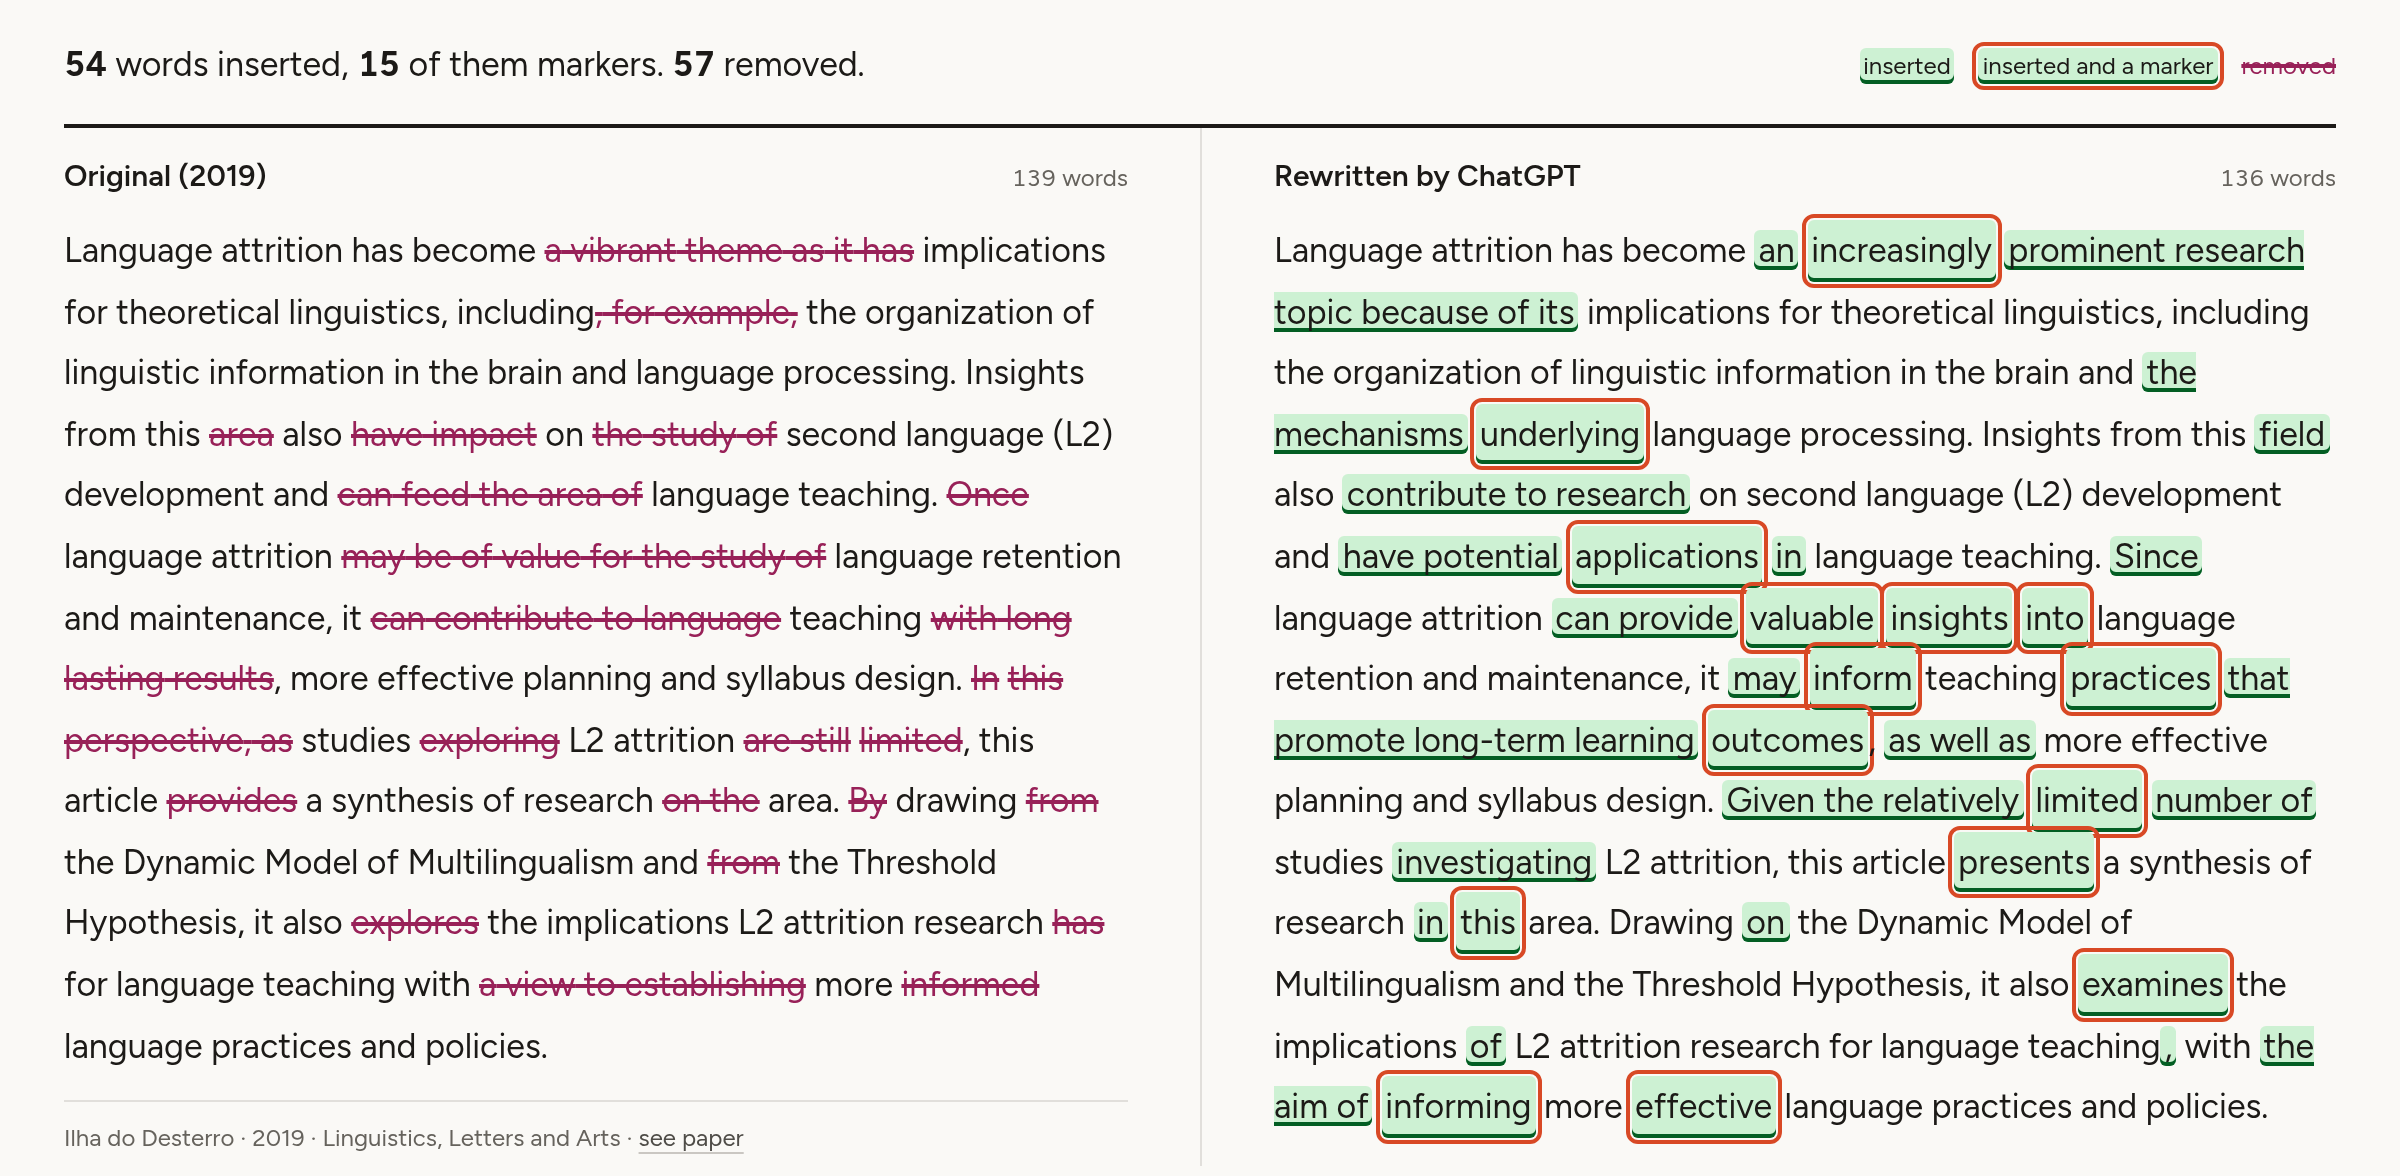
\includegraphics[width=0.78\textwidth]{figures/site-time-machine.png}
  \caption{ChatGPT inserts marker words when it polishes an abstract from 2019. Time machine screen
    of IAês. Left: the original, with the words ChatGPT removed struck through. Right: the rewrite,
    with inserted words in green and inserted words that are SciELO markers outlined.}
  \label{fig:site-time-machine}
\end{figure}

The experiment also shows that the markers catch an edit more easily in English. With the
cross-fitted sets of 2025, polishing raised the share of English abstracts with a marker by 29
(ChatGPT), 41 (Gemini) and 8 points (Claude), but the share of Portuguese abstracts by only 8, 14
and 0 points. This matters for H2, because similar rises in the two languages may hide more editing
of the Portuguese abstracts than of the English ones. The rates are too rough, however, to turn the
bound into an estimate of actual use, since one pass by a 2026 chatbot does not reproduce how the
tools were really used, with older models, repeated passes and drafting.

\subsection{Alternative explanations}
\label{sec:alternatives}

Chatbots are not the only possible source of these words. The method measures LLM-style vocabulary
and cannot tell which tool or person produced it. Machine translators, grammar checkers and human
editing services may leave such words too, and many of those tools now run on LLMs, so our results
refer to LLM-based tools in a broad sense (we did not test dedicated translators). Authors may also
pick up the words without any tool, as people did in speech \cite{yakura2024empirical}. We expect
this to be slower and smaller in formal writing than the sudden jumps we found, but we cannot rule
it out, and it would make the lower bound overstate the use of LLMs.

The other explanations we considered are handled by the design (Section~\ref{sec:excess-method}).
The balanced panels and the length reweighting remove the effect of journals that enter or leave
the corpus and of abstracts that grow longer. The panels hold only the journals that deposit
abstracts in Crossref regularly, which may differ from the rest, but the same-paper sample, drawn
from all the journals, shows rises in 2025 of about the size of the bounds. Policies that make some
journals publish in English only cannot explain the same-paper results either, since there every
paper has both abstracts.

\subsection{Discussion}
\label{sec:discussion}

Our reading of these results is that the share of SciELO abstracts touched by an LLM is probably
well above the lower bound. The bound counts only edits that leave a marker, and the experiment
shows that a polishing pass often leaves none, especially in Portuguese. Studies of full texts,
which give a chatbot more room to leave a trace, find signs of LLM influence in most articles of
2025 \cite{siler2026diffusion,holzwarth2026most}, and one of them estimates 53\% even for biomedical
abstracts of 2025 \cite{holzwarth2026most}. Our bounds are of the same order as those for the
Korean abstracts of 2025, which ranged from 10.5\% with single words to 20.6\% with a word set
chosen on half of the journals \cite{lee2026korean}.

We expected the English abstracts to carry most of the footprint, and they did not. Measured in
markers, the Portuguese footprint ended up close in size to the English one. English may have moved
first, as it did in Korean journals \cite{koo2026lexical,lee2026korean}, perhaps because the
pressure to publish in English made the English version the first one authors took to a chatbot,
but by 2025 the Portuguese abstracts had caught up. It seems that once authors adopt the tools,
they use them on both versions, directly or through translation.

The markers themselves change over time. The Portuguese \w{crucial} appeared in 1.63\% of the
abstracts of 2025 and in 0.79\% of those of 2026 so far. The partial year may explain part of the
drop, but it also fits the turnover of favored words described in Section~\ref{sec:vocab}. Anyone
who wants to keep monitoring will need to choose the marker sets anew each year.

One caution applies to everything above: a marker in a single abstract proves nothing. In 2021 and
2022, before ChatGPT, between 31\% and 39\% of the abstracts of the paired sample already contained
one of the 2025 or 2026 markers of their language, because many markers are ordinary words that
chatbots merely use more often. For this reason the site marks the words of a reader's own text
without passing judgment on it.

%%%%%%%%%%%%%%%%%%%%%%%%%%%%%%%%%%%%%%%%%%%%%%%%%%%%%%%%%%%%%%%%%%%%%%%%%%%%%%%%%%%%%%%%%%%%%%%%%%
\section{Conclusion}
\label{sec:conclusion}

LLM chatbots have left a measurable footprint in the abstracts of the SciELO Brazil journals that
deposit them in Crossref, in Portuguese as well as in English. H1 holds: from 2018 to 2022, no more
than six style words a year rose above their trend in either language, and in 2025, 108 did in
English and 69 in Portuguese. If the texts that no LLM touched kept to their trend, at least 17\% of
the English and 13\% of the Portuguese abstracts of 2025 went through an LLM. H2 is not supported.
Within the same papers, the English abstracts did not gain clearly more markers than the Portuguese
ones, although a lead of a few points remains possible. H3 holds only in part. The Portuguese
excess words are mostly style words, as expected, but they largely translate the English ones,
which refutes the claim that the two sets differ. The footprint also depends on the chatbot:
ChatGPT and Gemini added about five markers to each English abstract they polished, and Claude
about one.

The study has limitations, starting with the data. Crossref covers some journal-years and not
others, so the balanced panels of the main analyses hold only 84 to 181 of the 427 journals, which
may be more international than the rest, and 2026 runs only through October. We studied abstracts
only and set the Spanish ones aside. The corpus is about a hundred times smaller than PubMed, which
left the Portuguese marker sets of 2023 and 2024 nearly empty, and since words are counted in the
form in which they appear, a Portuguese verb spread over many forms may reach the thresholds later.

Some choices of method could be stricter. The split by DOI puts the same journals in both halves,
where a split by journal \cite{lee2026korean} would be more demanding. The style labels come from
an LLM whose agreement with a single annotator, the first author, who knew the hypotheses, was only
fair to moderate. In the H3 test, the controls match the markers in frequency only, so their parts
of speech may differ, and the words were translated without context. The experiment used 80 texts
per task, one pass and a different interface for each chatbot, and texts sent in the same
conversation may not be independent, which would make its intervals too narrow. Its markers also
come from a corpus in which ChatGPT was probably the most used chatbot.

Future work can extend the measurement to full texts, to the Spanish abstracts and to the other
SciELO collections, count Portuguese words by dictionary form, and calibrate the markers with
several models, prompts and passes, refreshing them with each model generation. It would also be
worth comparing measured use with the disclosures that SciELO and CNPq now ask for.

\subsection{Benefits and impacts of AI}
\label{sec:impacts}

For Brazilian science, the main benefit of chatbots is a lower cost of writing in English, a cost
that falls hardest on researchers who learned it as a second language
\cite{amano2023manifold,berdejoespinola2023ai}. The rise in output that followed LLM adoption was
largest among authors likely to be non-native English speakers \cite{kusumegi2026scientific}.
Chatbots also make bilingual publication cheaper, which may help journals keep publishing in
Portuguese. This study gained from LLMs in the same way: Claude labeled 1,682 excess words and
about 4,000 candidate control words and translated about 1,600 words, work that would have taken a
single researcher far longer.

The impact is already visible in our data. The change
reached the Portuguese abstracts nearly as much as the English ones, and it brought English word
choices with it, since most Portuguese markers translate English ones. If this continues, Brazilian
science may lose part of the variety of its styles
\cite{agarwal2025homogenize,sourati2026shrinking}, and its Portuguese may drift toward English
habits. Much of this use is also likely to go undisclosed, as it did elsewhere
\cite{gray2024contamination,kwon2025ok}. We do not think that detectors applied to single texts are
the answer, since they penalize the very authors who gain the most from the tools
\cite{liang2023gpt}. Disclosure, together with measurement over many texts at once, as we did here,
serves policy better, because it follows the impact without judging any single author.

\section*{Declaration of AI use}

The authors used Claude (Anthropic), through Claude Code with the Claude Opus 5.5 and Claude Fable
5.2 models, for three tasks: improving the writing of the text, with spelling corrections and more
fluent phrasing; searching the literature through deep search with the Exa search engine; and
speeding up the development of the code of the IAês site. As part of the method
(Section~\ref{sec:method}), Claude Opus 5.5 labeled and translated words, and ChatGPT, Gemini and
Claude Sonnet 5.5 rewrote and translated abstracts in the experiment. The authors take full
responsibility for the content of this paper.

\bibliographystyle{sbc}
\bibliography{references}

\end{document}
